\subsection{Propriedade}

Assim como a comparação realizada anteriormente, que abordou o que é um método
comparando-o com os conceitos da programação estruturada, seguindo a mesma
analogia, uma propriedade (também conhecida como atributo, variável membro ou ainda variável
de instância) pode ser considerada como os dados que um objeto possuí,
descrevendo desta forma, as características que a ele pertencem
\cite{programmingPhp}.

Sendo assim, os atributos são variáveis que estão definidas dentro de uma
classe, deste modo, geralmente são acessados através de uma interface de acesso,
pois não estão visíveis para que outros objetos manipulem os dados diretamente,
se isto ocorresse, poderia comprometer a segurança da informação e também o
conceito de que cada objeto possuí uma finalidade.

Então, uma propriedade (pensando na classe Carro) poderia ser uma característica
que um carro possuí no mundo real. Portanto, é possível levantar de acordo com
o nosso conhecimento rapidamente os seguintes parâmetros que definem um carro:
cor, quantidade de portas, possuí direção hidráulica, etc.

Na Figura \ref{fig:propriedade}, é apresentada a sintaxe para definição de duas
propriedades (cor e quantidade de portas) da classe Carro implementadas na
linguagem \acs{PHP}.

\begin{figure}[h!tb]
	\caption{Criação de propriedades na linguagem PHP}
	\label{fig:propriedade}

	\centering
	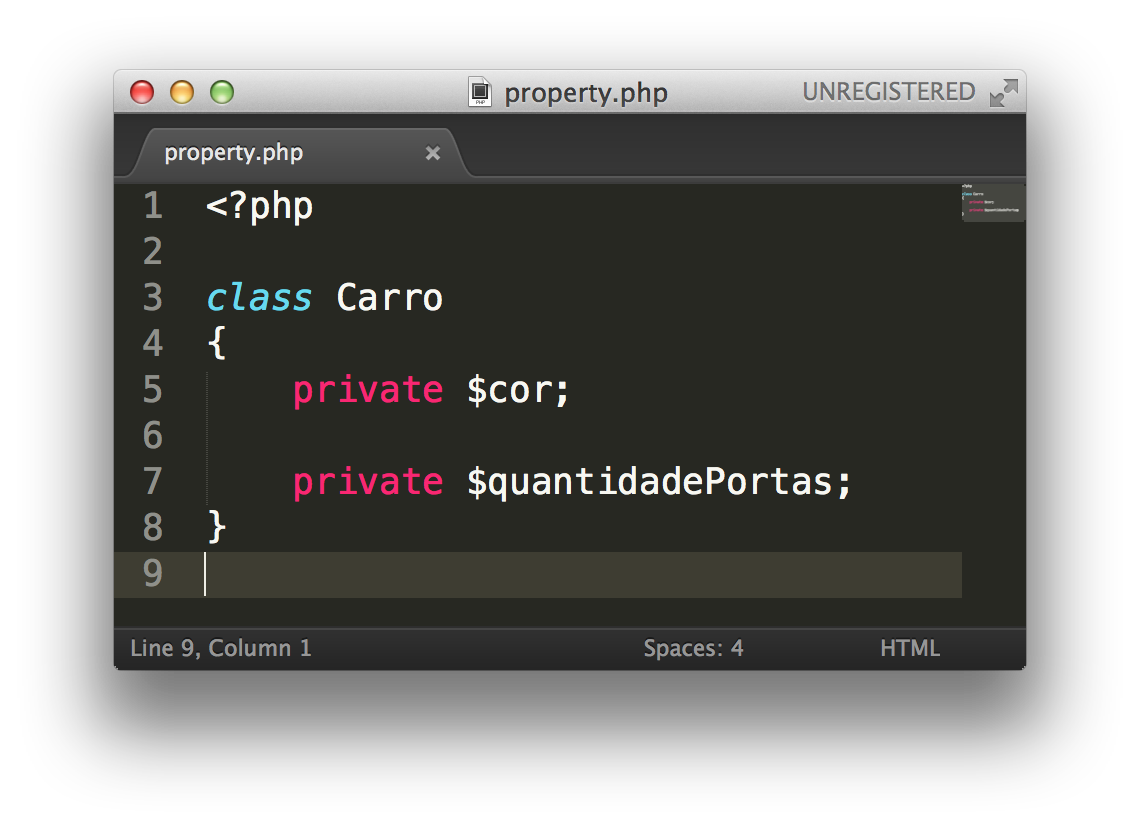
\includegraphics[width=0.75\textwidth]{images/property.png}

	\centering
	\footnotesize Fonte: \fonteOAutor
\end{figure}

\FloatBarrier 	% Este comando impede que as imagens
				% flutuem a partir deste ponto no seu documento

Por conseguinte, abaixo será apresentada a análise das linhas de código
exibidas na Figura \ref{fig:propriedade}:

\begin{alineas}
    \item linha 1: vê-se o início da execução de um bloco de código PHP;
    \item linha 3: define-se uma classe chamada \textit{Carro};
    \item linha 5: utiliza-se uma palavra reservada \textbf{private} que se
    refere a visibilidade da propriedade no contexto de um conjunto de objetos
    (mais detalhes serão apresentadas adiante) e, em seguida, é definido o nome
    de uma variável, que neste caso chama-se \textbf{\$cor};
    \item linha 7: é definida uma segunda propriedade para a classe
    Carro chamada de \textbf{\$quantidadePortas};
    \item linha 8: informa-se onde termina o bloco que compreende a
    classe \textit{Carro}.
\end{alineas}

\subsubsection{Propriedade estática}

Como foi visto anteriormente, as classes são formadas por variáveis de instância
e métodos. Entretanto, as variáveis que forem declaradas com a palavra reservada
\textit{static}, serão compartilhadas por toda a classe. Por conta disto, as
variáveis que assim forem definidas, recebem o nome de variáveis estáticas ou ainda
propriedades estáticas \cite{learningJava}.

Conforme afirma \citeonline{c++ComoProgramar}, a palavra chave \textit{static}
é utilizada quando as informações precisam ser compartilhadas por todas
as instância e não apenas em um único objeto.

Na Figura \ref{fig:propriedadeEstatica} é exibido um exemplo de propriedade
estática utilizando a linguagem \acs{PHP}.

\begin{figure}[h!tb]
	\caption{Propriedade estática definida na linguagem PHP}
	\label{fig:propriedadeEstatica}

	\centering
	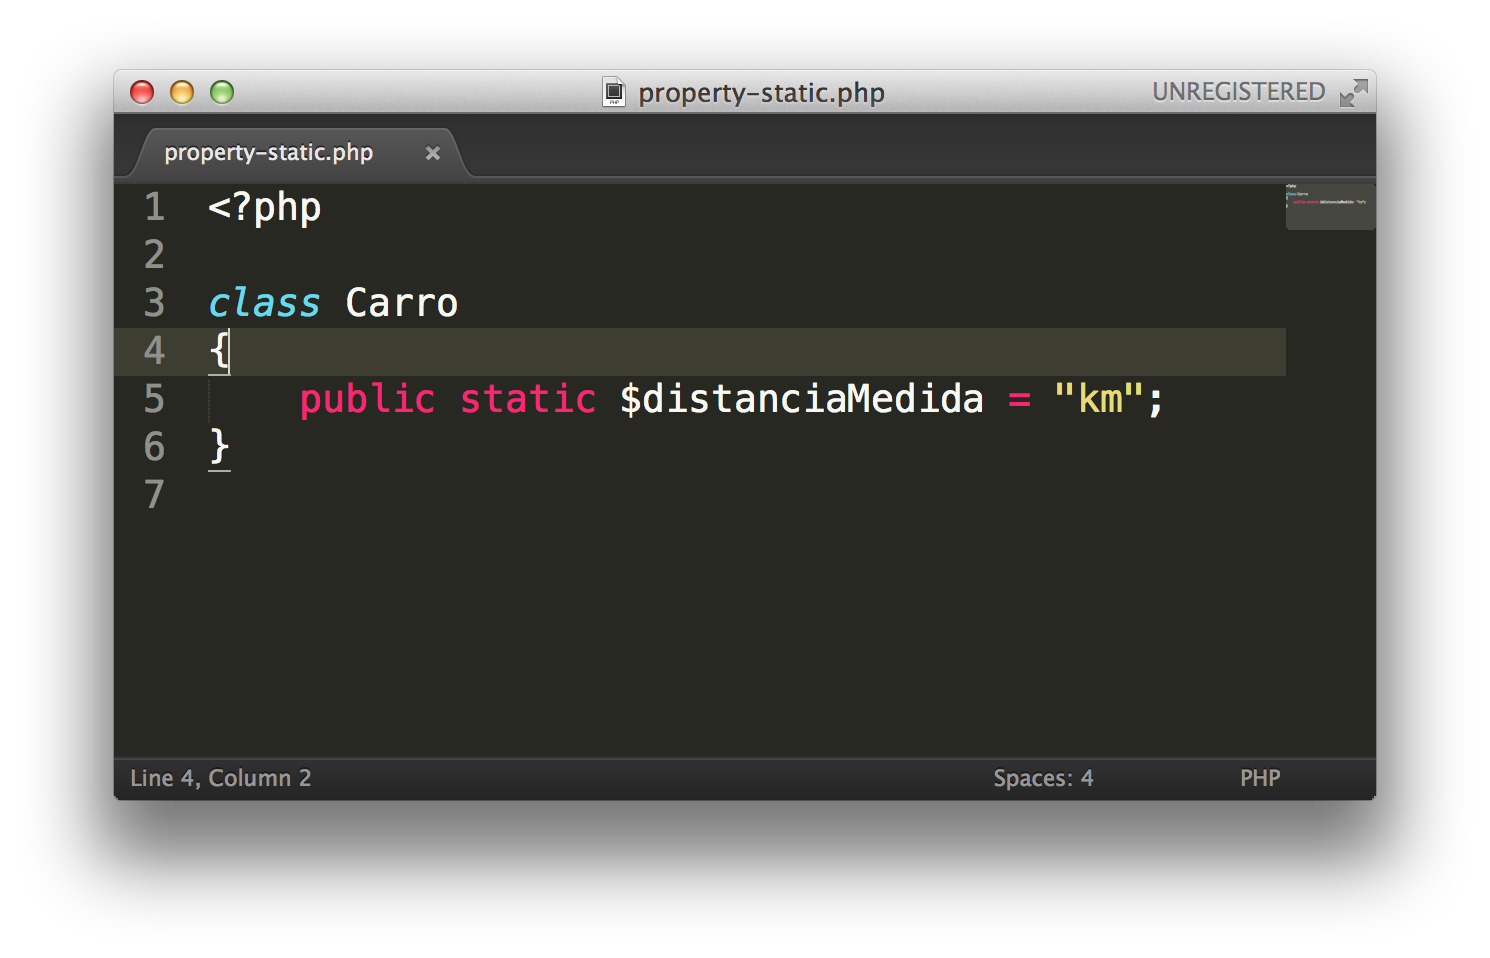
\includegraphics[width=0.82\textwidth]{images/property-static.png}

	\centering
	\footnotesize Fonte: \fonteOAutor
\end{figure}

\FloatBarrier 	% Este comando impede que as imagens
				% flutuem a partir deste ponto no seu documento

A seguir, é apresentado em detalhes as linhas de código exibidas na Figura
\ref{fig:propriedadeEstatica}:

\begin{alineas}
    \item linha 1: vê-se o início da execução de um bloco de código PHP;
    \item linha 5: define-se a propriedade estática que armazenará a unidade de
    medida utilizada por todos os veículos, que neste caso é \textit{km}
    (quilômetros).
\end{alineas}

A seguir será apresentado o conceito que define o que é uma constante e
exibido um exemplo de uso implementado na linguagem \acs{PHP}.
